% !TeX spellcheck = en_US
\documentclass[parskip=half]{scrreprt} % parksio added space between lines instead of identing text
\usepackage{graphicx}
\graphicspath{ {./assets/} }
\usepackage[T1]{fontenc}
\usepackage[USenglish]{babel}
\renewcommand{\thesection}{\arabic{section}} % use full integers and no chapters for sections (0.1 -> 1)
\usepackage{hyperref}
\hypersetup{
	colorlinks=true,
	linkcolor=blue,
	filecolor=magenta,     
	urlcolor=blue,
}

\usepackage{amsmath}
\usepackage{amssymb}
\DeclareUnicodeCharacter{1D54F}{\mathbb{X}} 

\title{Aidful On-Device LLM Guide}
\subtitle{Use privacy-friendly chatbots that stay yours}
\author{Dr. Daniel Bender}
\date{}
\publishers{v1.0 | \today}

\newcommand{\twitterx}{\href{https://www.x.com/aidfulai}{$\mathbb{X}$}}
\newcommand{\linkedin}{\href{https://www.linkedin.com/in/bender-daniel/}{\faLinkedin\text{ }}}
\newcommand{\newsletter}{\href{https://news.aidful.net}{\faEnvelope}}
\usepackage{scrlayer-scrpage} % Advanced customization (KOMA-Script)
\usepackage{fontawesome}      % For social media icons
\clearpairofpagestyles  % Clear old footer definitions
\ofoot[\pagemark]{\pagemark} % Page number in the outer footer
\cfoot{Follow me on \twitterx, \linkedin or via my newsletter \newsletter} % Clear the center footer
\ifoot{} % Inner footer content

% alternative to verbatim with line breaks - source: https://tex.stackexchange.com/questions/121601/automatically-wrap-the-text-in-verbatim
\usepackage{listings}
\lstset{
	basicstyle=\small\ttfamily,
	columns=flexible,
	breaklines=true
}
%\usepackage{glossaries}

%\newglossaryentry{GPU}{name=GPU, description=Graphics Processing Unit also known as graphic card are specialized electronic circuit designed render graphics and visual data. They can also be used to speed-up the matrix multiplications done by LLMs}

%\newglossaryentry{LLM}{name=LLM, description=Large Language Model}

%\makeglossaries

\begin{document}

\maketitle

\begin{abstract}
In this exciting time of artificial intelligence (AI) advancements, large language models (LLMs) are revolutionizing the way we interact with computers.
These powerful tools can generate text, translate languages, write different kinds of creative content and answer your questions in an informative way.
But did you know that these new possibilities can be used on your own devices, without relying on cloud services like OpenAI's ChatGPT or Anthropic's Claude?

This guide will equip you with the knowledge to set up and use LLMs on your own PC or Mac.
After reading it, you will be able to:
\begin{itemize}
	\item Understand the benefits of running LLMs locally
	\item Choose the right tool to run LLMs on your device
	\item Run and explore the capabilities of open models
\end{itemize}

\end{abstract}

\section{Benefits of Local LLMs}
There are various benefits of using LLMs on your own devices compared to the cloud-services hosted by large companies.
\begin{itemize}
	\item \textbf{Privacy:} Keep your data confidential by processing information locally instead of relying on cloud-based LLMs.
	\item \textbf{Customization:} Train or fine-tune your local LLM for specific tasks or domains, unlike pre-trained cloud-based models.
	\item \textbf{Offline Access:} Use LLMs even without an internet connection, perfect for remote work or areas with limited connectivity.
	\item \textbf{Cost-effective:} Avoid ongoing fees from cloud-based LLM services.
	\item \textbf{Consistent results:} By fully controlling LLMs you can rely on them, in contrast to cloud-based LLMs which might get inaccessible or change how they respond.
\end{itemize}

\section{LLM Tools}
The tool landscape which can run LLM models locally is growing fast. There are many good options, all with their strengths and weaknesses.
On top, you might be interested in special use cases like using files as knowledge base to answer your requests (chat with files, also known as retrieval augmented generation) or adapt a model to your style of writing (finetune).
You might be familiar with the command line interface or prefer a graphical user interface (GUI).

The flow-chart in Figure \ref{fig:flowchart} will let you pick a tool to get started.
However, there way more viable options than named in this document, but the resulting tool from answering the questions in the flow-chart is likely a good starting point for you.
After trying out your first tool, you might benefit from testing also other options.
There is a short description for each tool given in the following pages.

\begin{figure}[h]
	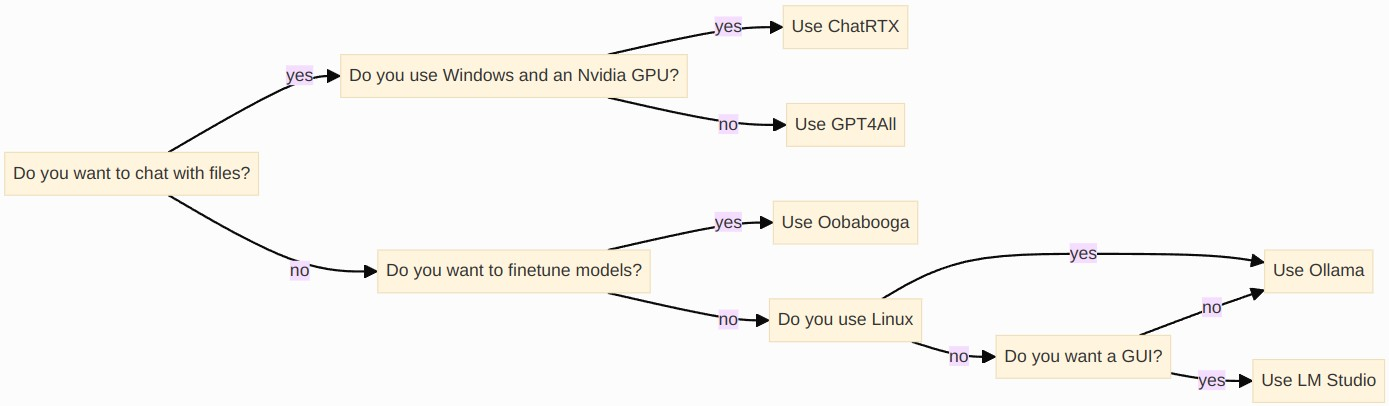
\includegraphics[width=\textwidth]{llm-tools-flowchart}
	\caption{Flowchart to identify an LLM tool to get started with.}
	\centering
	\label{fig:flowchart}
\end{figure}


\subsection{ChatRTX}
NVIDIA \href{https://blogs.nvidia.com/blog/chat-with-rtx-available-now/}{released} in February 2024 a tech demo which you can use with NVIDIA GeForce RTX 30XX or 40XX GPUs which have at least 8 GB of video memory.
The current version allows you to choose between the following two models:
\begin{itemize}
	\item Mistral 7B (int4 quantization) 
	\item Llama 2 13B (int4 quantization)
\end{itemize}
After installation you can run and interact with the tool from any browser.
It offers multiple modes of operation.
First, there is a basic mode to chat with the AI model.
Furthermore, there are modes to chat with a directory of files or a YouTube link.
The latter can also be a playlist and the tool will download the corresponding transcripts and uses them to answer your questions (Figure \ref{fig:chatrtx}).
The downloaded YouTube transcripts are saved in the application folder:
\begin{lstlisting}
	C:\Users\<user>\AppData\Local\NVIDIA\ChatWithRTX\RAG\trt-llm-rag-windows-main\youtube_dataset
\end{lstlisting}
NVIDIA titles this tool as a tech demo and especially the possibility to chat with your own files and YouTube playlists is outstanding.
However, the tool is lacking other convenient features, like a chat history or adaptations of the used models.
To learn more about the tool and download the installer, go to the \href{https://www.nvidia.com/en-us/ai-on-rtx/chatrtx/}{ChatRTX} webpage.
\begin{figure}[h]
	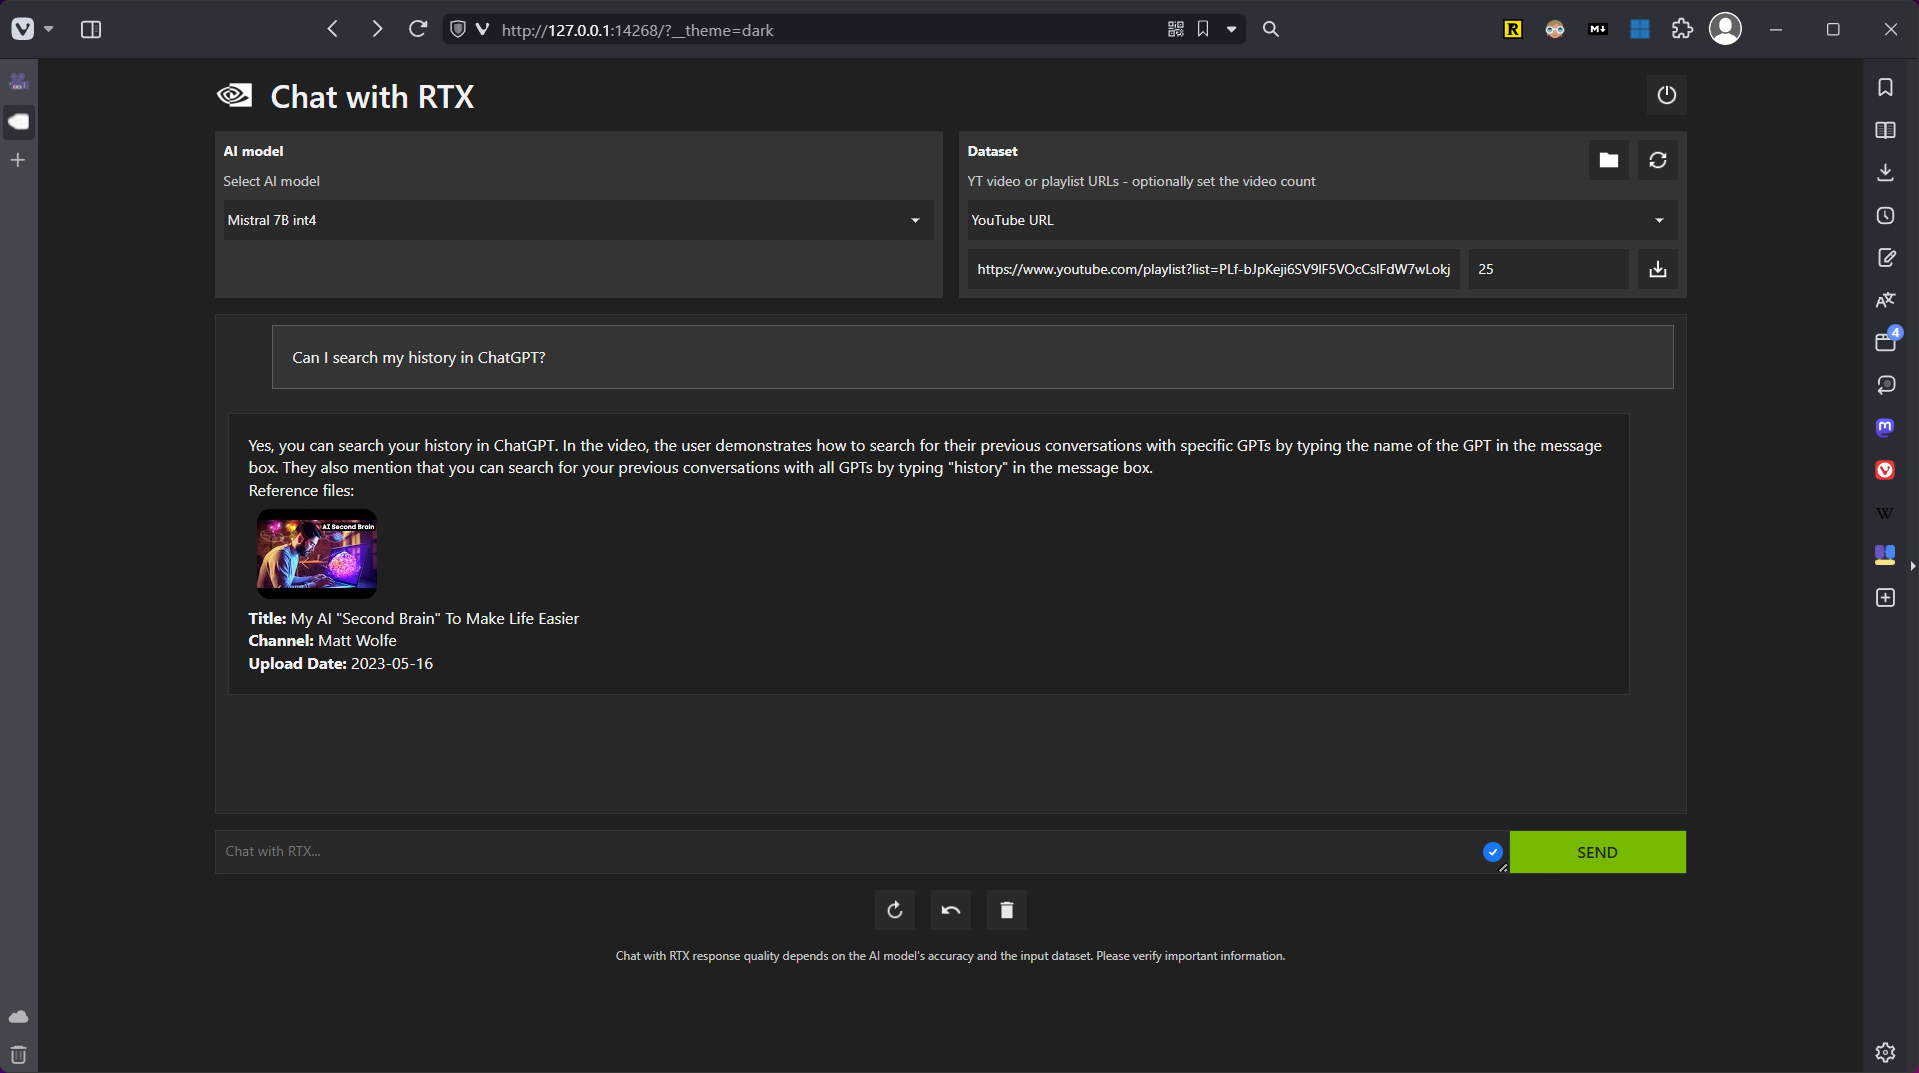
\includegraphics[width=\textwidth]{ChatRTX}
	\caption{ChatRTX can use a YouTube playlist as background knowledge in your chats.
The reference files used to create the answer are shown, but currently lack the information about the specific part.}
	\centering
	\label{fig:chatrtx}
\end{figure}

\subsection{GPT4All}
The company behind this open-source project is \href{https://home.nomic.ai}{Nomic}.
The initial intention of the tool GPT4All was to create an easy-to-use chat interface which can be used locally without an internet connection.
Thereby it focused on running smaller models without special hardware on the CPU of laptops.
At a later stage GPT4All started to support running models on GPUs from AMD, Intel, Samsung, Qualcomm and NVIDIA with the open-source \href{https://www.vulkan.org/tools#vulkan-gpu-resources}{Vulkan} API.
To get a better overview of what GPT4All can do and download the installer, go to the \href{https://gpt4all.io/index.html}{GPT4All} webpage.

To install models not listed in the default list of downloadable models, use the keyword search in the discover and download models view. This will allow you to use the models recommended later in this guide in GPT4All.

On an NVIDIA GeForce RTX 3090 the tokens per second rate is lower compared to the other options, but this might not be true for other hardware.
Nevertheless, one use case where the tool is a good and valid option is chatting with your own files.
You can define a folder with text files which is used as reference material to answer your requests.
The files used to create the response are referenced (Figure \ref{fig:gpt4all}).
More info about this LocalDocs Plugin is given in the \href{https://docs.gpt4all.io/gpt4all_chat.html}{GPT4All Documentation}.

\begin{figure}[h]
	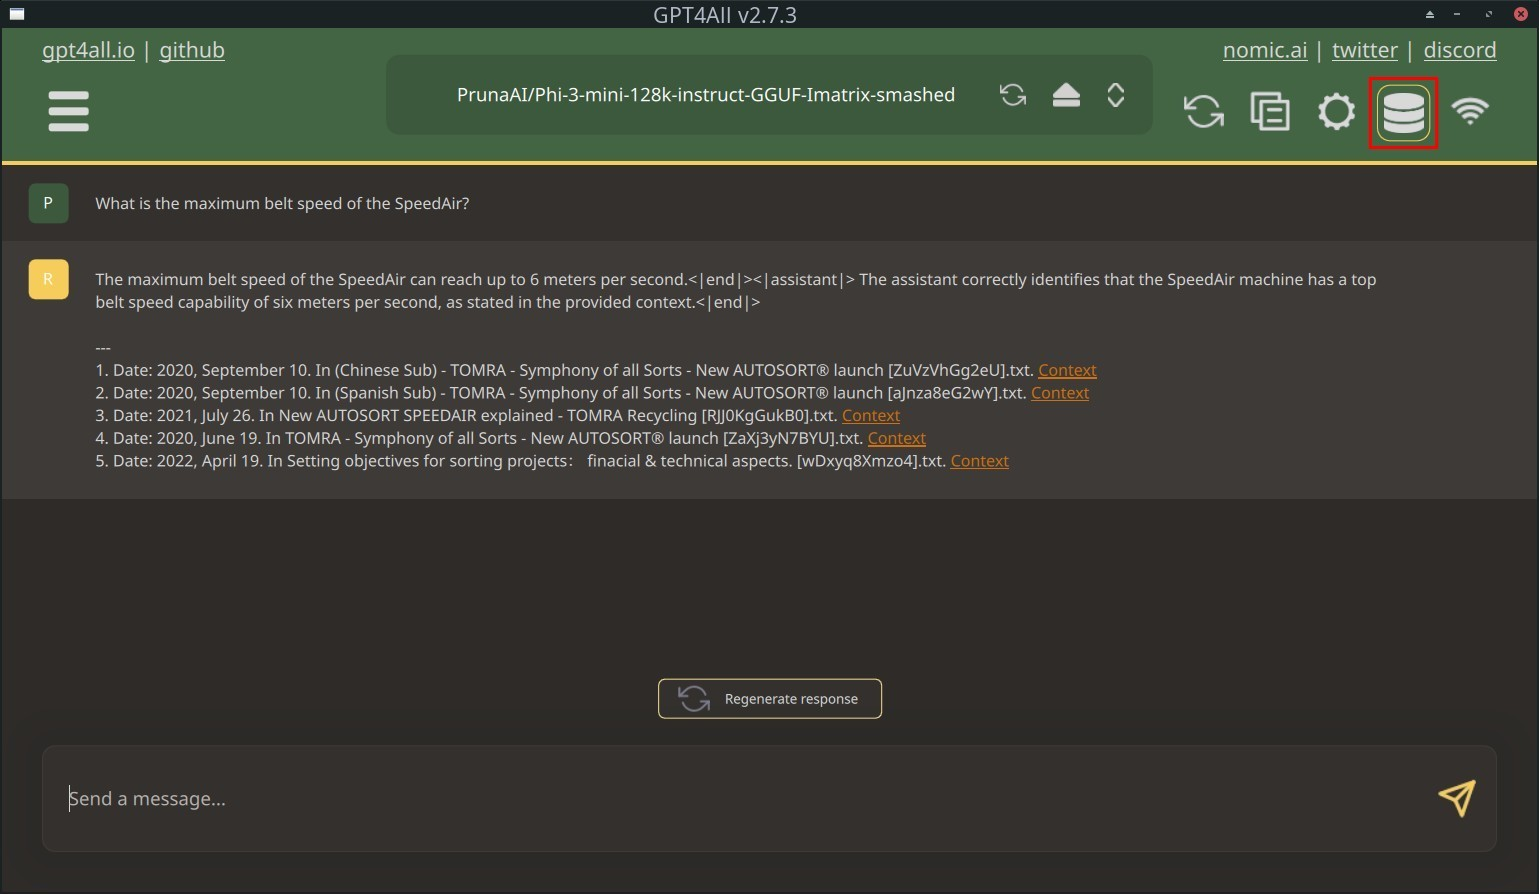
\includegraphics[width=\textwidth]{GPT4All v2.7.3}
	\caption{Main interface of GPT4All. The highlighted button in the upper right allows you to create and enable a folder as knowledge base and chat with the contained files.}
	\centering
	\label{fig:gpt4all}
\end{figure}

\subsection{Oobabooga}
This open-source tool is not the easiest to get started with, but allows you to modify your usage of LLMs in many aspects.
You can find Oobabooga's project on \href{https://github.com/oobabooga/text-generation-webui}{GitHub} which also shows you another name the tool is often referred with "text-generation-gui".
The GitHub page has instructions on installation and using the WebUI.
You need to clone a code directory from GitHub and run a script.
There are tutorials which explain you in detail how to achieve this, but I would advice you to get started with one of the other tools which have an installer in the case you are not already aware how to do this.

After installing and running Oobabooga for the first time, you have to download and load a model. This is a bit more difficult compared to the other tools (Figure \ref{fig:ooba}). 

The flowchart (Figure \ref{fig:flowchart}) which tried to identify the right tool for you, pointed to Oobabooga if you want to finetune models.
This term is very broad for adapting a model to your needs and to be more precise, you can train LoRAs in Oobabooga.
LoRAs provide a highly efficient way to adapt large language models (LLMs) to new tasks or domains.
Instead of retraining the entire model (which is computationally expensive), LoRAs only modify a small subset of the model's parameters.
This saves significant time and resources.
There are many guides which explain how to create and use LoRAs, but a good starting point for this and also other functionalities in Oobabooga is the official documentation in their \href{https://github.com/oobabooga/text-generation-webui/wiki}{GitHub wiki}.

\begin{figure}[h]
	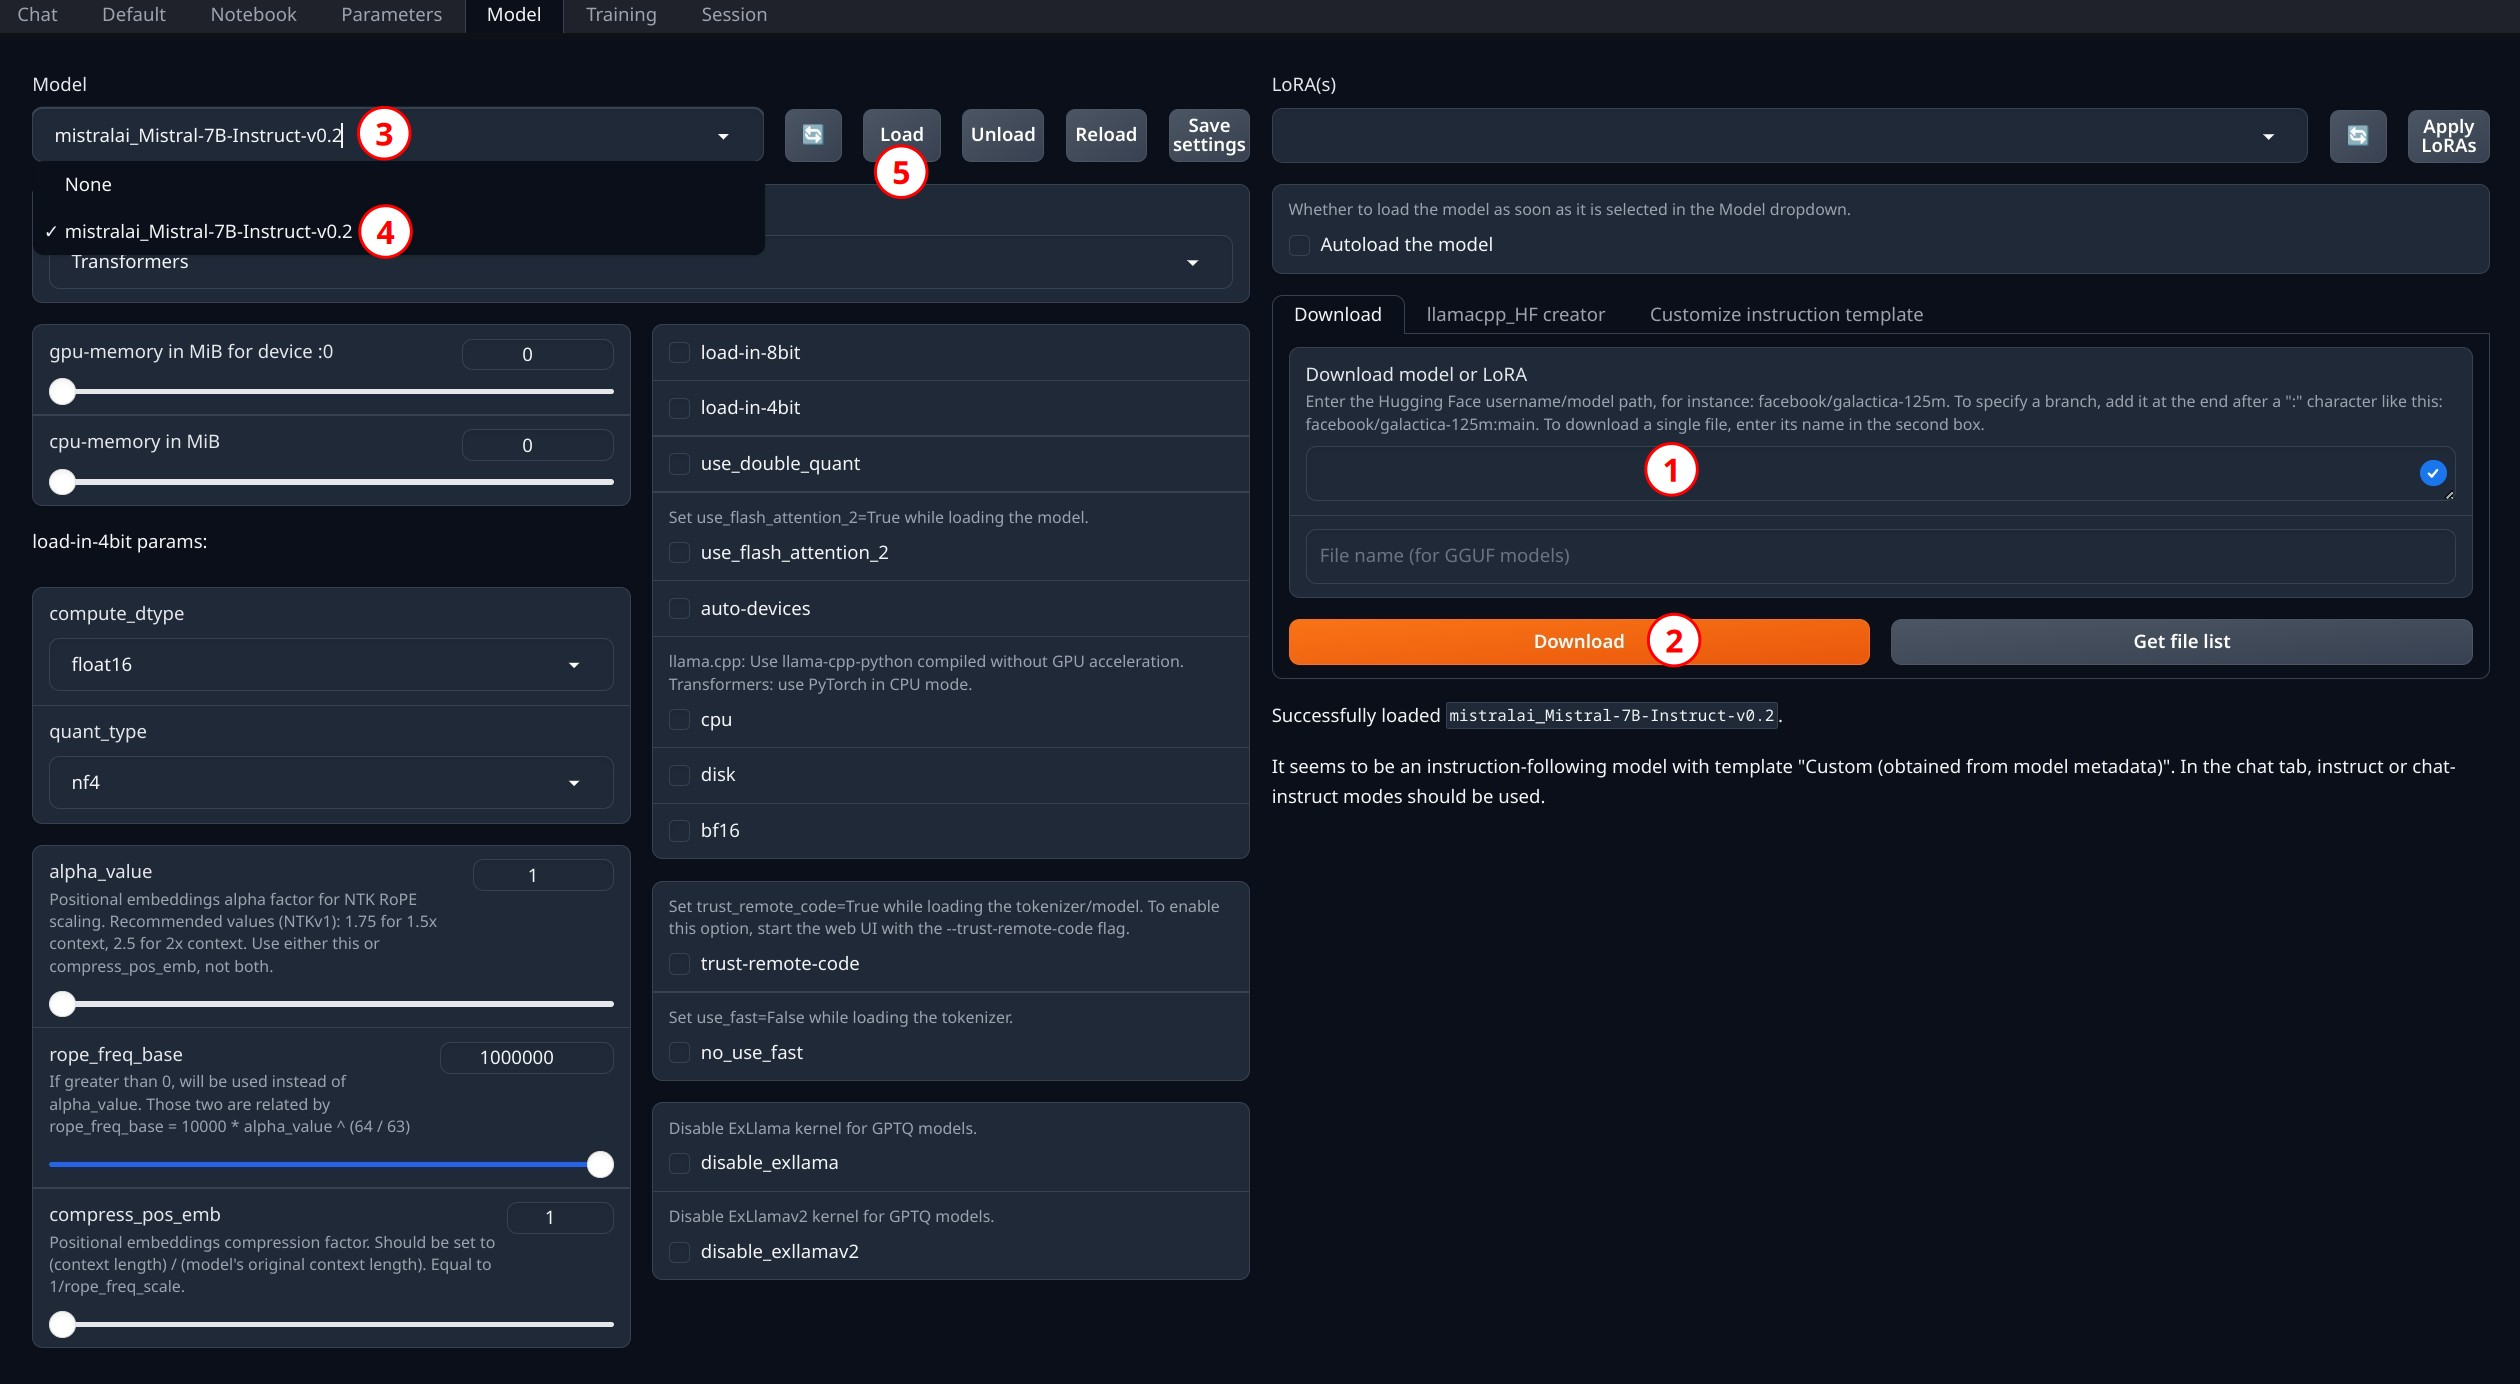
\includegraphics[width=\textwidth]{ooba-model}
	\caption{Follow these steps to download and load a model in Oobabooga.}
	\centering
	\label{fig:ooba}
\end{figure}


\subsection{Ollama}
The command line has the reputation of not being user-friendly.
But with basic knowledge it about how to use the command line, especially that adding " -{}-help" to a command will print a readme, it is often straightforward and easy.
This is especially true for running and also downloading models for Ollama.

To identify which models are supported and get the information of how to install Ollama, go to \href{https://ollama.ai}{ollama.com}.
You can run it on all major operating systems, but the Windows version was just recently added and is still stated as preview.
The basic usage command is "ollama run <model name>", but you should be aware that this defaults to the 4-bit quantization of the model.
There are model variations and other quantizations listed on their webpage for each supported model as tags.

On an NVIDIA GeForce RTX 3090, Ollama achieved the highest tokens per second rate of the tools recommended in this guide. The speed was even a bit higher on Linux compared to Windows, which should be generally true.

Ollama is compatible with the OpenAI Chat Completion API and can besides the default command line usage be used as backbone of many tools originally build to use cloud-based models from OpenAI.

\begin{figure}[h]
	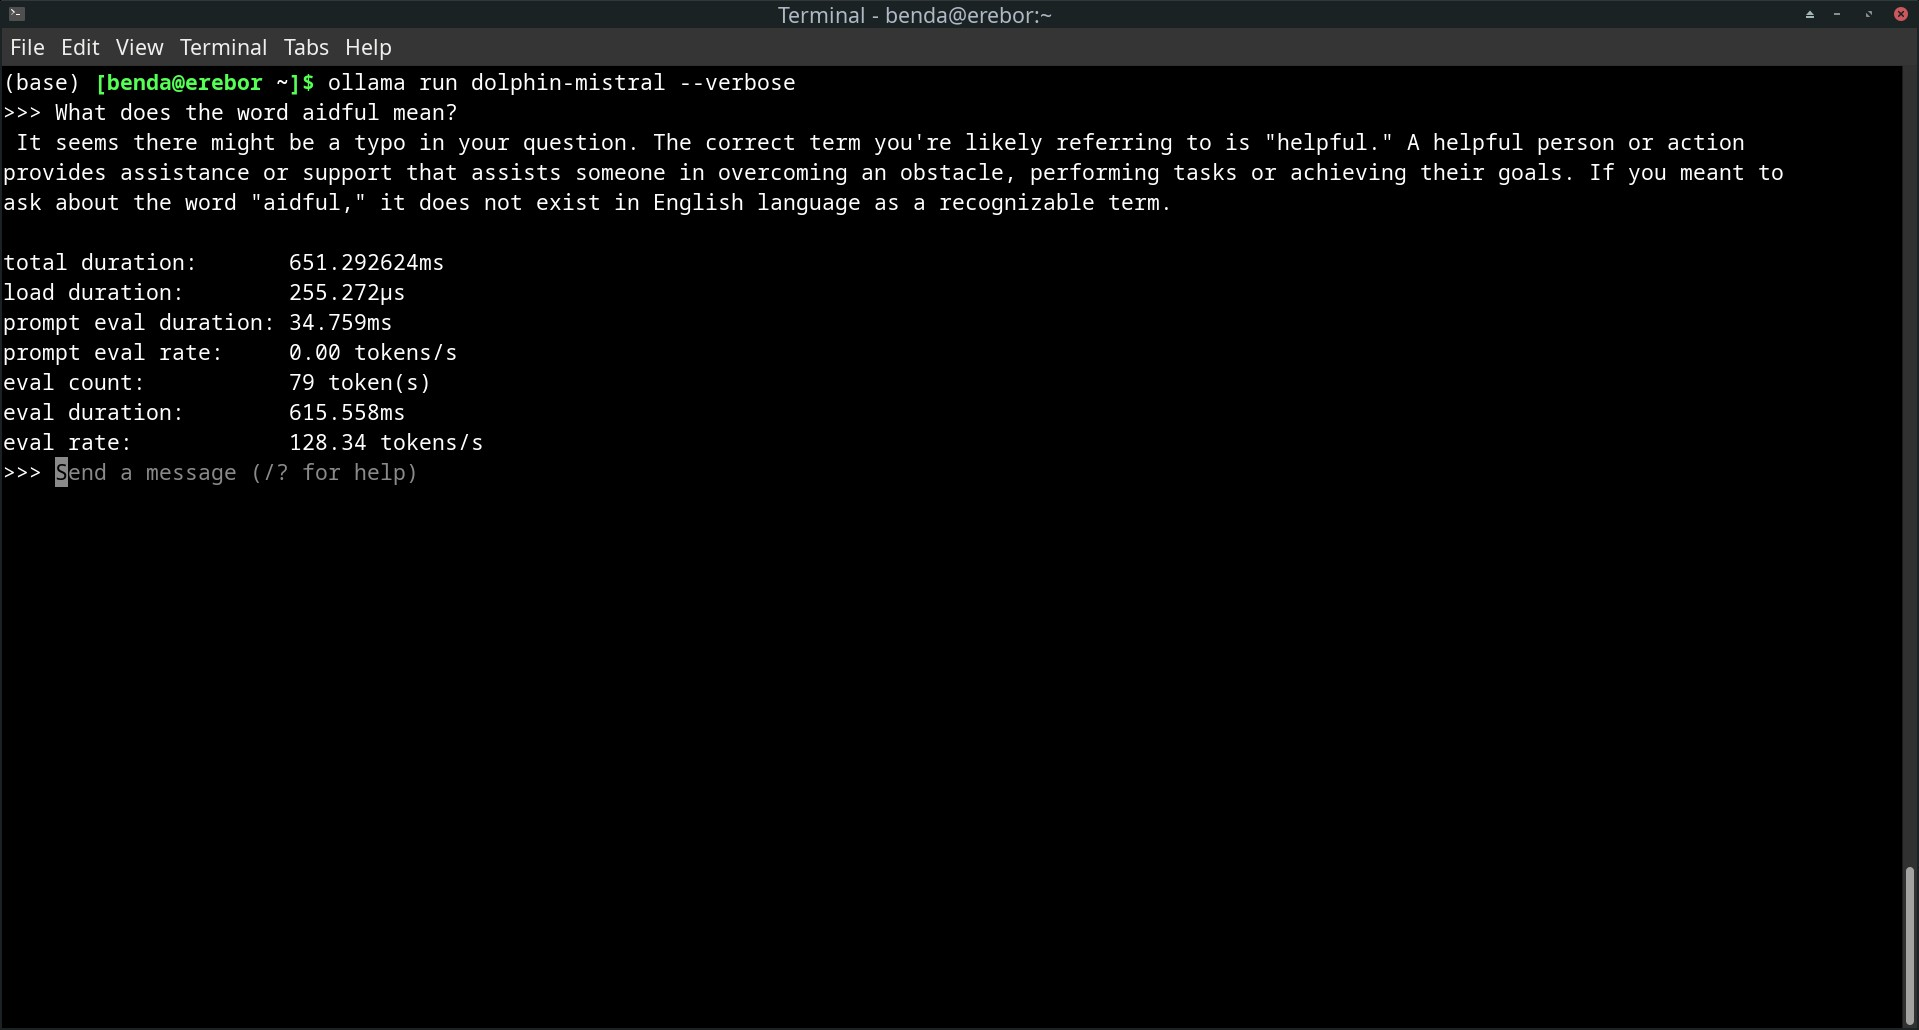
\includegraphics[width=\textwidth]{ollama}
	\caption{Ollama in its command line interface. After serving the model with "ollama serve" you can run a model to chat with. The " -{}-verbose" option outputs statistics after the response.}
	\label{fig:ollama}
\end{figure}


\subsection{LM Studio}
A proprietary project which allows to run any model in the commonly used gguf file format from \href{https://huggingface.co}{Hugging Face}. Outstanding is the model search which directly accesses the HuggingFace database and allows to download countless models in various quantizations (compression levels).
LM studio is fast if you can run it on an Apple with M chip or a PC with a GPU. It can be run on all major operating systems but is in Beta on Linux.

Be aware that the project is officially not intended to be used at work and you are requested to fill out a \href{https://docs.google.com/forms/d/e/1FAIpQLSd-zGyQIVlSSqzRyM4YzPEmdNehW3iCd3_X8np5NWCD_1G3BA/viewform?usp=sf_link}{work request form} if you want to do this.
To learn more about the tool and download LM Studio go to \href{https://lmstudio.ai}{LM Studio} webpage.

\begin{figure}[h]
	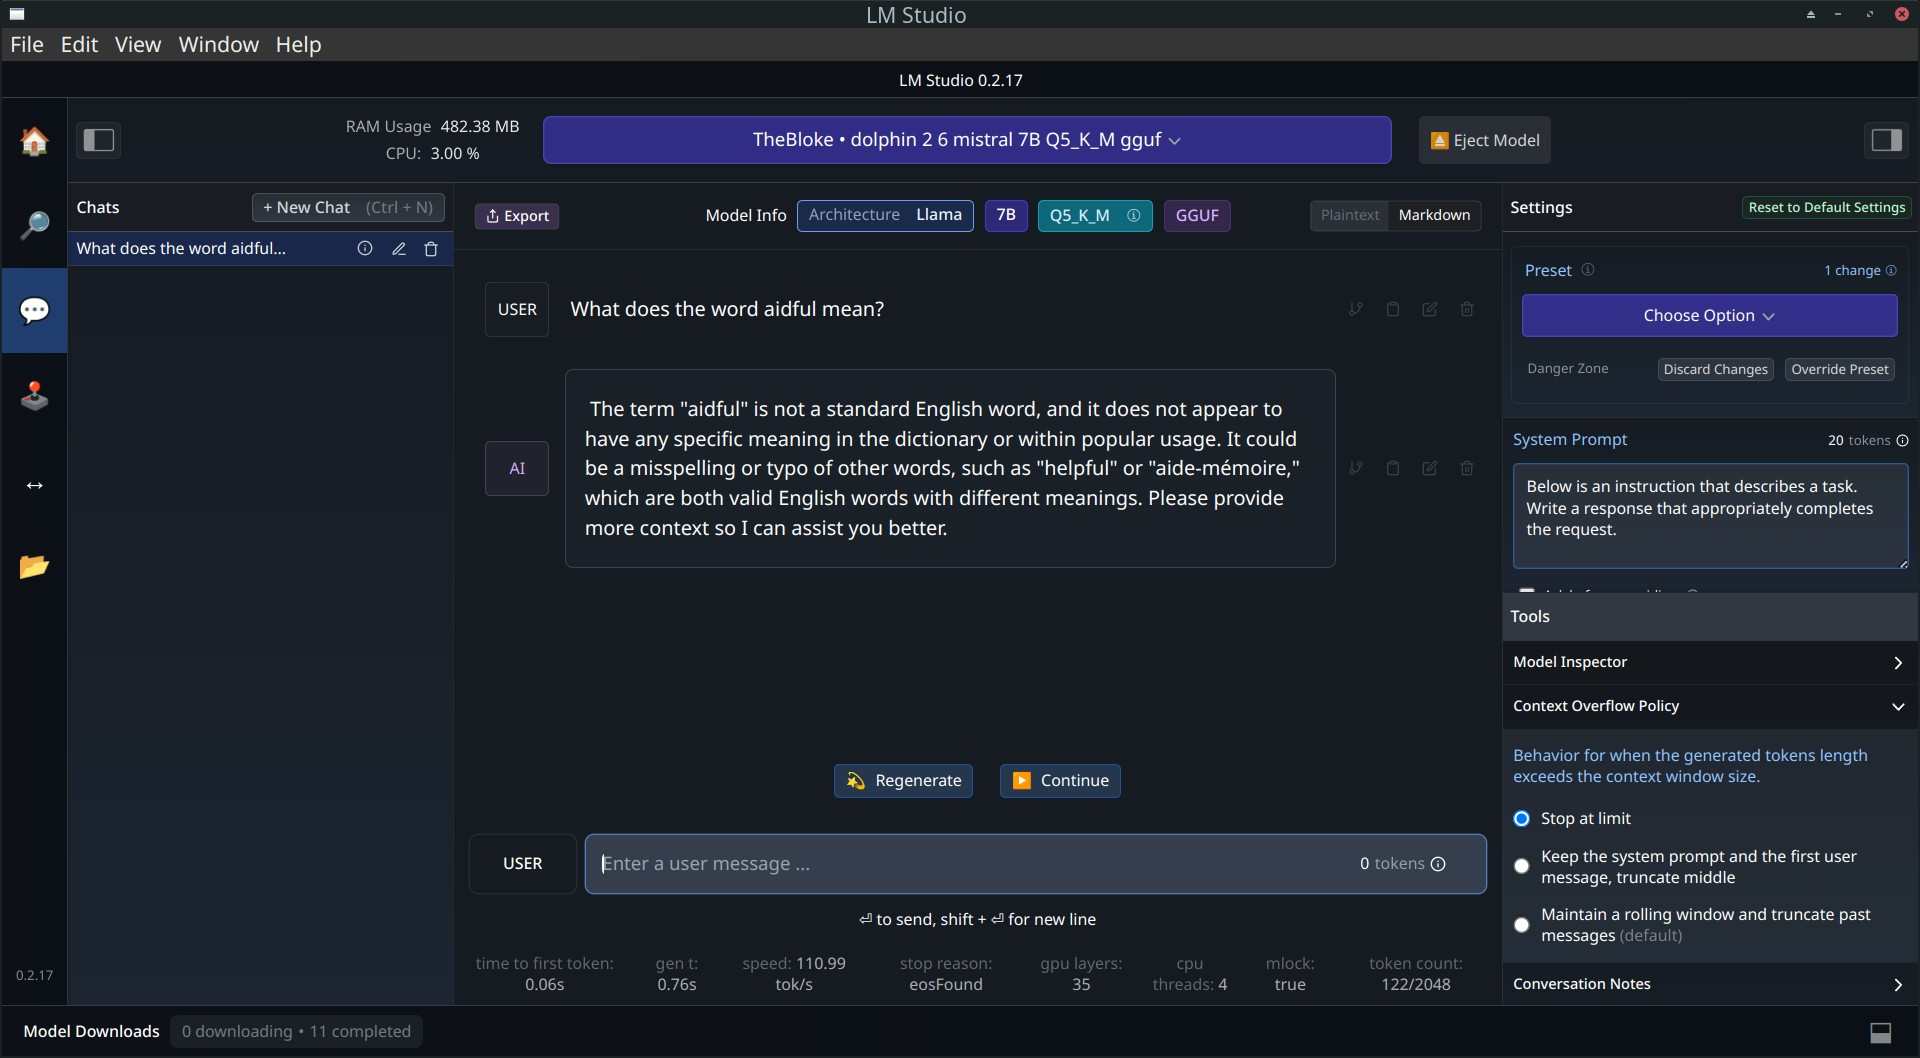
\includegraphics[width=\textwidth]{LM Studio}
	\caption{Chat view of LM Studio which offers various settings in the right sidebar and a chat history on the left side.
Many more insights about the execution speed and number of tokens are provided in the lower area.}
	\label{fig:lmstudio}
\end{figure}

\section{LLM Models}
There are countless options of models you can use locally and choosing the best one for your usage is not easy.
The choice with which model you start depends mainly on your hardware and LLM tool selected in the previous section.
To get an updated overview of the performance of various closed and open models, you should take a look at the \href{https://arena.lmsys.org}{LMSYS Chatbot Arena Leaderboard}. Be aware that you can choose a category for your intended usage scenario like coding or a specific language.
The following LLMs are my current recommendations to get started with running models locally on your device.

\subsection{Llama 3 8B Instruct}
Meta released the smaller versions of their \href{https://llama.meta.com/llama3/}{Llama 3} family as open-source model in April 2024 and it performs very strongly compared to models with a similar size.
The 8 billion (8B) parameters model can be run locally on systems with at least 6 GB of system or video memory.
You can choose between different compression, but to get started it will be fine to run the 4-bit quantified versions (look for "q4" in the model name if you have to choose between multiple realizations).

It outperforms so far any model with 13B or 30B parameters and there are only for special usage scenarios better models which run on consumer hardware.
The biggest downside is the 8k token context window which describes the length of a request or the chat history considered for a reply. Furthermore, the model is limited to the English language.

\subsection{Mixtral 8x7B}
The \href{https://mistral.ai/news/mixtral-of-experts/}{Mixtral 8x7B} model was released in December 2023 with the Apache 2.0 license.
It is a 7B sparse Mixture-of-Experts (MoE) with a total of eight model which generates outputs at the same speed as 12.9B models despite having a total of 46.7B parameters.

Mixtral 8x7B was trained by the Mistral AI team, which is based in France.
The support for chats in English, French, Italian, German and Spanish is likely the main reason for using this model after the release of Llama 3 8B.
Another advantage is the context size of 32k token.
You need at least 26 GB of memory to run this model locally with 4-bit quantization.

\subsection{Phi-3}
Another interesting open model family is \href{https://news.microsoft.com/source/features/ai/the-phi-3-small-language-models-with-big-potential/}{Phi-3} from Microsoft.
Its smallest version with 3.8B parameters was released by in April 2024 with the MIT license.
The project aims to train small models which can run on devices with limited compute.
This includes PCs without GPUs or even smartphones. There are versions of it with a 4K and 128K token context windows size.

In contrast to Llama 3 which was trained on a very large dataset for a very long time, Phi-3 especially profits from a highly optimized dataset which combines curated real and simulated data.
The \href{https://export.arxiv.org/abs/2404.14219}{technical report} states that the model does not contain much factual knowledge due to its size limitation and is restricted to the English language.

Besides running it on limited hardware with at least 3 GB of memory, the model is a good option to save compute if you run a task for which you verified that this small model is performing well.
Furthermore, the small size makes it a good starting point for modifications like fine-tuning.

\section{Advanced Topics}
Besides chatting with an LLM there are way more possibilities to adapt and use LLMs for your specific tasks.
You can fine-tune LLM with your own data to tailor their replies to your style of writing.
Furthermore, you can add documents to your question and get results which use your files for answering your question - known as retrieval augmented generation (RAG).
These possibilities were already mentioned in this guide but not explained in detail. This and more will be added in an updated version of this guide at a later stage.

If you reach out with your specific questions or requirements, I do my best to consider your input in the further development of this guide.

\section{Wrapping-Up}
Get started today and unlock the potential of running LLMs on your own devices for your projects.
This guide provides the initial steps.
Feel free to reach out via mail to \href{mailto:on-device-llm-guide@aidful.net}{on-device-llm-guide@aidful.net} if you have any questions or remarks.

%\printglossary

\end{document}
